% --- LaTeX Lecture Notes Template - S. Venkatraman ---

% --- Set document class and font size ---

\documentclass[letterpaper, 12pt]{article}

% --- Package imports ---

% Vietnamese support
\usepackage[vietnamese]{babel}

% Bibliography support
\usepackage{biblatex}
\addbibresource{Citations.bib}

% Extended set of colors
\usepackage[dvipsnames, table, xcdraw]{xcolor}

\usepackage{
  amsmath, amsthm, amssymb, mathtools, dsfont, units,          % Math typesetting
  graphicx, wrapfig, subfig, float,                            % Figures and graphics formatting
  listings, color, inconsolata, pythonhighlight,               % Code formatting
  fancyhdr, sectsty, hyperref, enumerate, enumitem, framed }   % Headers/footers, section fonts, links, lists

% lipsum is just for generating placeholder text and can be removed
\usepackage{hyperref, lipsum} 

% --- Fonts ---

\usepackage{newpxtext, newpxmath, inconsolata}

% --- Page layout settings ---

% Set page margins
\usepackage[left=1.35in, right=1.35in, top=1.0in, bottom=.9in, headsep=.2in, footskip=0.35in]{geometry}

% Anchor footnotes to the bottom of the page
\usepackage[bottom]{footmisc}

% Set line spacing
\renewcommand{\baselinestretch}{1.2}

% Set spacing between paragraphs
\setlength{\parskip}{1.3mm}
\setlength{\parindent}{0pt}

% Allow multi-line equations to break onto the next page
\allowdisplaybreaks

% --- Page formatting settings ---

% Set image captions to be italicized
\usepackage[font={it,footnotesize}]{caption}

% Set link colors for labeled items (blue), citations (red), URLs (orange)
\hypersetup{colorlinks=true, linkcolor=RoyalBlue, citecolor=RedOrange, urlcolor=ForestGreen}

% Set font size for section titles (\large) and subtitles (\normalsize) 
\usepackage{titlesec}
\titleformat{\section}{\large\bfseries}{{\fontsize{19}{19}\selectfont\textreferencemark}\;\; }{0em}{}
\titleformat{\subsection}{\normalsize\bfseries\selectfont}{\thesubsection\;\;\;}{0em}{}

% Enumerated/bulleted lists: make numbers/bullets flush left
%\setlist[enumerate]{wide=2pt, leftmargin=16pt, labelwidth=0pt}
\setlist[itemize]{wide=0pt, leftmargin=16pt, labelwidth=10pt, align=left}

% --- Table of contents settings ---

\usepackage[subfigure]{tocloft}

% Reduce spacing between sections in table of contents
\setlength{\cftbeforesecskip}{.9ex}

% Remove indentation for sections
\cftsetindents{section}{0em}{0em}

% Set font size (\large) for table of contents title
\renewcommand{\cfttoctitlefont}{\large\bfseries}

% Remove numbers/bullets from section titles in table of contents
\makeatletter
\renewcommand{\cftsecpresnum}{\begin{lrbox}{\@tempboxa}}
\renewcommand{\cftsecaftersnum}{\end{lrbox}}
\makeatother

% --- Set path for images ---

\graphicspath{{Images/}{../Images/}}

% --- Math/Statistics commands ---

% Add a reference number to a single line of a multi-line equation
% Usage: "\numberthis\label{labelNameHere}" in an align or gather environment
\newcommand\numberthis{\addtocounter{equation}{1}\tag{\theequation}}

% Shortcut for bold text in math mode, e.g. $\b{X}$
\let\b\mathbf

% Shortcut for bold Greek letters, e.g. $\bg{\beta}$
\let\bg\boldsymbol

% Shortcut for calligraphic script, e.g. %\mc{M}$
\let\mc\mathcal

% \mathscr{(letter here)} is sometimes used to denote vector spaces
\usepackage[mathscr]{euscript}

% Convergence: right arrow with optional text on top
% E.g. $\converge[p]$ for converges in probability
\newcommand{\converge}[1][]{\xrightarrow{#1}}

% Weak convergence: harpoon symbol with optional text on top
% E.g. $\wconverge[n\to\infty]$
\newcommand{\wconverge}[1][]{\stackrel{#1}{\rightharpoonup}}

% Equality: equals sign with optional text on top
% E.g. $X \equals[d] Y$ for equality in distribution
\newcommand{\equals}[1][]{\stackrel{\smash{#1}}{=}}

% Normal distribution: arguments are the mean and variance
% E.g. $\normal{\mu}{\sigma}$
\newcommand{\normal}[2]{\mathcal{N}\left(#1,#2\right)}

% Uniform distribution: arguments are the left and right endpoints
% E.g. $\unif{0}{1}$
\newcommand{\unif}[2]{\text{Uniform}(#1,#2)}

% Independent and identically distributed random variables
% E.g. $ X_1,...,X_n \iid \normal{0}{1}$
\newcommand{\iid}{\stackrel{\smash{\text{iid}}}{\sim}}

% Sequences (this shortcut is mostly to reduce finger strain for small hands)
% E.g. to write $\{A_n\}_{n\geq 1}$, do $\bk{A_n}{n\geq 1}$
\newcommand{\bk}[2]{\{#1\}_{#2}}

% Math mode symbols for common sets and spaces. Example usage: $\R$
\newcommand{\R}{\mathbb{R}}	% Real numbers
\newcommand{\C}{\mathbb{C}}	% Complex numbers
\newcommand{\Q}{\mathbb{Q}}	% Rational numbers
\newcommand{\Z}{\mathbb{Z}}	% Integers
\newcommand{\N}{\mathbb{N}}	% Natural numbers
\newcommand{\F}{\mathcal{F}}	% Calligraphic F for a sigma algebra
\newcommand{\El}{\mathcal{L}}	% Calligraphic L, e.g. for L^p spaces

% Math mode symbols for probability
\newcommand{\pr}{\mathbb{P}}	% Probability measure
\newcommand{\E}{\mathbb{E}}	% Expectation, e.g. $\E(X)$
\newcommand{\var}{\text{Var}}	% Variance, e.g. $\var(X)$
\newcommand{\cov}{\text{Cov}}	% Covariance, e.g. $\cov(X,Y)$
\newcommand{\corr}{\text{Corr}}	% Correlation, e.g. $\corr(X,Y)$
\newcommand{\B}{\mathcal{B}}	% Borel sigma-algebra

% Other miscellaneous symbols
\newcommand{\tth}{\text{th}}	% Non-italicized 'th', e.g. $n^\tth$
\newcommand{\Oh}{\mathcal{O}}	% Big-O notation, e.g. $\O(n)$
\newcommand{\1}{\mathds{1}}	% Indicator function, e.g. $\1_A$

% Additional commands for math mode
\DeclareMathOperator*{\argmax}{argmax}		% Argmax, e.g. $\argmax_{x\in[0,1]} f(x)$
\DeclareMathOperator*{\argmin}{argmin}		% Argmin, e.g. $\argmin_{x\in[0,1]} f(x)$
\DeclareMathOperator*{\spann}{Span}		% Span, e.g. $\spann\{X_1,...,X_n\}$
\DeclareMathOperator*{\bias}{Bias}		% Bias, e.g. $\bias(\hat\theta)$
\DeclareMathOperator*{\ran}{ran}			% Range of an operator, e.g. $\ran(T) 
\DeclareMathOperator*{\dv}{d\!}			% Non-italicized 'with respect to', e.g. $\int f(x) \dv x$
\DeclareMathOperator*{\diag}{diag}		% Diagonal of a matrix, e.g. $\diag(M)$
\DeclareMathOperator*{\trace}{trace}		% Trace of a matrix, e.g. $\trace(M)$
\DeclareMathOperator*{\supp}{supp}		% Support of a function, e.g., $\supp(f)$

% Numbered theorem, lemma, etc. settings - e.g., a definition, lemma, and theorem appearing in that 
% order in Lecture 2 will be numbered Definition 2.1, Lemma 2.2, Theorem 2.3. 
% Example usage: \begin{theorem}[Name of theorem] Theorem statement \end{theorem}
\theoremstyle{definition}
\newtheorem{theorem}{Theorem}[section]
\newtheorem{proposition}[theorem]{Proposition}
\newtheorem{lemma}[theorem]{Lemma}
\newtheorem{corollary}[theorem]{Corollary}
\newtheorem{definition}[theorem]{Definition}
\newtheorem{example}[theorem]{Example}
\newtheorem{remark}[theorem]{Remark}

% Un-numbered theorem, lemma, etc. settings
% Example usage: \begin{lemma*}[Name of lemma] Lemma statement \end{lemma*}
\newtheorem*{theorem*}{Theorem}
\newtheorem*{proposition*}{Proposition}
\newtheorem*{lemma*}{Lemma}
\newtheorem*{corollary*}{Corollary}
\newtheorem*{definition*}{Definition}
\newtheorem*{example*}{Example}
\newtheorem*{remark*}{Remark}
\newtheorem*{claim}{Claim}

% --- Left/right header text (to appear on every page) ---

% Do not include a line under header or above footer
\pagestyle{fancy}
\renewcommand{\footrulewidth}{0pt}
\renewcommand{\headrulewidth}{0pt}

% Right header text: Lecture number and title
\renewcommand{\sectionmark}[1]{\markright{#1} }
\fancyhead[R]{\small\textit{\nouppercase{\rightmark}}}

% Left header text: Short course title, hyperlinked to table of contents
\fancyhead[L]{\hyperref[sec:contents]{\small Ôn tập VLDC2}}

% --- Document starts here ---

\begin{document}

% --- Main title and subtitle ---

\title{Đề cương ôn tập VLDC2 \\[1em]
\normalsize }

% --- Author and date of last update ---

% \author{\normalsize Your name here}
% \date{\normalsize\vspace{-1ex} Last updated: \today}

% --- Add title and table of contents ---

\maketitle
\tableofcontents\label{sec:contents}

% --- Main content: import lectures as subfiles ---

% First argument to \section is the title that will go in the table of contents. Second argument is the title that will be printed on the page.
\section[Chương 1]{Chương 1: Điện trường}

\subsection{Câu 1}

\begin{itemize}
  \item Điện trường là loại môi trường đặc biệt được tạo ra xung quanh các hạt mang điện tích, có tính chất gây lực tác dụng lên các điện tích đặt trong nó
  \item Vecto cường độ điện trường tại 1 điểm là đại lượng có giá trị bằng lực tác dụng của điện trường lên một đơn vị điện tích dương tại điểm đó
  \begin{itemize}
    \item Vecto cddt gây bởi 1 điện tích điểm: $\vec{E} = \frac{\vec{F}}{q_0} = \frac{q}{4\pi\epsilon_0\epsilon r^3} \vec{r}$
    \item Vecto cddt gây bởi 1 hệ điện tích điểm: $\vec{E} = \frac{\vec{F}}{q_0} = \frac{\sum\limits \vec{F}_i}{q_0} = \sum\limits \frac{\vec{F}_i}{q_0} = \sum\limits \vec{E}_i \Rightarrow$  Nguyên lý chồng chất điện trường
    \item Vecto cddt gây bởi 1 vật mang điện: Chia nhỏ vật thành các phần nhở chứa điện tích $dq$. Coi vật như một hệ vô số điện tích điểm: $\vec{E} = \int d\vec{E} = \int \frac{dq}{4\pi\epsilon_0\epsilon r^2} \frac{\vec{r}}{r}$
  \end{itemize}
\end{itemize}

\subsection{Câu 2}

\begin{itemize}
  \item Đường cảm ứng điện là đường cong mà tiếp tuyến tại mỗi điểm trùng với phương của vecto cảm ứng điện tại điểm đó, chiều của đường cảm ứng điện là chiều của $\vec{D}$.
  \item ĐIểm khác nhau: Đường sức điện trường biểu diễn cho $\vec{E}$, đường cảm ứng điện biểu diễn cho $\vec{D} \Rightarrow$ Đường cảm ứng điện đi qua mặt phân cách các môi trường là đường liên tục
  \item Thông lượng cảm ứng qua diện tích $S$:
  \begin{itemize}
    \item Giả sử diện tích $S$ trong 1 điện trường $\vec{D}$. Chia nhỏ $S$ thành các phần $dS$ sao cho $\vec{D}$ tại mỗi điểm trên $dS$ là như nhau
    \item $d\Phi = \vec{D}d\vec{S} = DdS\cos\alpha = DdS_n \Rightarrow \Phi = \int_S d\Phi = \int_S \vec{D}d\vec{S}$
  \end{itemize}
  \item Góc khối $d\Omega = \frac{dS\cos\alpha}{r^2}$, điện thông qua 1 mặt $d\Phi = \vec{D}d\vec{S} = \frac{q}{4\pi r^3} \vec{r}d\vec{S} = \frac{q}{4\pi} \frac{dS\cos\alpha}{r^2} = \frac{q}{4\pi} d\Omega$
  \item Điện thông qua 1 mặt bao quanh $q$: $\Phi = \oint_S d\Phi = q$
\end{itemize}

\subsection{Câu 3}

\begin{itemize}
  \item Lưỡng cực điện là 1 hệ 2 điện tích điểm bằng nhau về trị số nhưng trái dấu, cách nhau 1 khoảng rất nhỏ so với khoảng cách tới các điểm ta xét
  \item Momen lưỡng cực điện $\vec{p}_e = q\vec{l}$ 
  \item Ý nghĩa: Biết được $\vec{p}_e$ có thể biết được $\vec{E}$ do lưỡng cực điện gây ra. Vậy ta nói $\vec{p}_e$ đặc trưng cho tính chất điện của lưỡng cực
  \item Xác định $E$ tại điểm $M$ nằm trên trung trực và cách xa 2 điểm 1 khoảng $r$ (tự làm)
\end{itemize}

\begin{equation*}
  \vec{E}_m = - \frac{\vec{p}_e}{4\pi\epsilon_0\epsilon r^3}
\end{equation*}

\subsection{Câu 4}\label{def:o-g}

\begin{itemize}
  \item Định lý O-G trong điện trường: Điện thông gửi qua một mặt kín có giá trị bằng tổng đại số các điện tích trong mặt kín đó.
  \item Dạng tích phân: $$\Phi = \oint_S \vec{D}d\vec{S} = \sum\limits q_i$$
  \item Dạng vi phân: $$\text{div}\,\vec{D} = \rho$$
  \item Áp dụng với mặt phẳng vô hạn mật độ $\sigma$:
  \begin{itemize}
    \item Xét hình trụ với đáy $\Delta S$, song song mp. $\vec{D}$ vuông góc với mp đó
    \item Tính ra được $D = \frac{\sigma}{2}$
  \end{itemize}
  \item Cddt trong tụ phẳng: $E = \frac{\sigma}{\epsilon_0\epsilon} = \frac{q}{\epsilon_0\epsilon S}$
\end{itemize}

\subsection{Câu 5}

\begin{itemize}
  \item O-G như \hyperref[def:o-g]{trên}
  \item Áp dụng với mặt trụ dài vô hạn, bán kính R, mật độ $\sigma$
  \begin{itemize}
    \item Xét hình trụ ngoài với bán kính $r > R$ (tự làm)
    \item Tính được $E = \frac{\lambda}{2\pi r}$
  \end{itemize}
\end{itemize}

\subsection{Câu 6}

\begin{itemize}
  \item O-G như \hyperref[def:o-g]{trên}
  \item Áp dụng với mặt cầu bán kính $R$ tại điểm nằm ngoài cách $r > R$:
  \begin{itemize}
    \item Xét một mặt cầu ngoài với bán kính $r > R$ (tự làm)
    \item Tính được $E = \frac{q}{4\pi\epsilon_0\epsilon r^2}$
  \end{itemize}
\end{itemize}

\subsection{Câu 7}

\begin{itemize}
  \item Tính công của lực tĩnh điện trong chuyển dời:
  \begin{itemize}
    \item Xét công của lực điện trên một chuyển dời nhỏ $ds$:
    \begin{equation*}
      dA = \vec{F}d\vec{s} = q_0 \frac{q}{4\pi\epsilon_0\epsilon r^3} \vec{r}d\vec{s} = \dots = \frac{q_0qdr}{4\pi\epsilon_0\epsilon r^2}
    \end{equation*}
    \item Công của lực trong chuyển dời từ $M$ đến $N$:
    \begin{equation*}
      A = \int_{M}^{N} dA = \int_{r_M}^{r_N} \frac{q_0q}{4\pi\epsilon_0\epsilon} \frac{dr}{r^2} = \frac{q_0q}{4\pi\epsilon_0\epsilon r_M} - \frac{q_0q}{4\pi\epsilon_0\epsilon r_N}
    \end{equation*}
  \end{itemize}
  \item Trường tĩnh điện gọi là trường thế vì công của lực điện trong sự chuyển dời một điện tích điểm $q_0$ trong điện trường không phụ thuộc vào dạng của đường cong dịch chuyển mà chỉ phụ thuộc vào điểm đầu và cuối của chuyển dời
  \item Lưu số vector cddt dọc theo 1 đường cong kín bằng 0
  \begin{equation*}
    \oint \vec{E}d\vec{s} = 0
  \end{equation*}
\end{itemize}

\subsection{Câu 8}

\begin{itemize}
  \item Thế năng của điện trường tại một điểm là đại lượng đặc trưng cho điện trường tại điểm đang xét.
  \item Thế năng điện trường có trị số bằng giá trị của thế năng của một đơn vị điện tích dương tại điểm đang xét 
  \begin{equation*}
    V = \frac{W}{q_0}
  \end{equation*}
  \item Điện thế tại một điểm trong điện trường (quy ước $W_\infty = 0$): 
  \begin{equation*}
    V = \frac{W}{q_0} = \frac{q}{4\pi\epsilon_0\epsilon r}
  \end{equation*}
  \item Điện thế trong một hệ điện tích điểm:
  \begin{equation*}
    V = \sum V_i = \sum \frac{q_i}{4\pi\epsilon_0\epsilon r_i}
  \end{equation*}
  \item Điện thế trong một điện trường bất kỳ:
  \begin{equation*}
    V_M = \frac{W_M}{q_0} = \int_{M}^{\infty} \vec{E}d\vec{s}
  \end{equation*}
\end{itemize}

\section[Chương 2]{Chương 2: Vật dẫn}

\subsection{Câu 1}

Điều kiện cân bằng tĩnh điện của vật dẫn mang điện:

\begin{enumerate}
  \item Vector cường độ điện trường tại mọi điểm trong vật dẫn bằng 0
  \begin{equation*}
    \vec{E}_{tr} = 0
  \end{equation*}
  \item Thành phần tiếp tuyến của vector cường độ điện trường tại mọi điểm trên mặt vật dẫn bằng 0
  \begin{equation*}
    \vec{E}_t = 0, \vec{E}_n = \vec{E}
  \end{equation*}
\end{enumerate}

Các tính chất của vật dẫn tích điện cân bằng:

\begin{enumerate}
  \item Vật dẫn là vật đẳng thế
  \begin{itemize}
    \item Xét 2 điểm $M, N$ trên vật dẫn:
    \begin{equation*}
      V_M - V_N = \int_{M}^{N} \vec{E}d\vec{s} = \int_{M}^{N} E_sds
    \end{equation*}
    \item Bên trong vật dẫn thì $E_s = 0$ nên $V$ tại mọi điểm bên trong bằng nhau
    \item Bên ngoài vật dẫn thì $E_s = E_t = 0$ nên $V$ tại mọi điểm ngoài bằng nhau
    \item Vì $V$ có tính liên tục nên $V$ tại mọi điểm như nhau
  \end{itemize}
  \item Khi vật dẫn ở trạng thái cân bằng tĩnh điện, điện tích chỉ phân bố ở bên ngoài vật dẫn. Bên trong điện tích bằng 0
  \begin{itemize}
    \item Xét 1 mặt kín $S$ bất kỳ bên trong vật dẫn. Theo O-G có
    \begin{equation*}
      \sum q_i = \oint_S \vec{D}d\vec{s}
    \end{equation*}
    \item Bên trong vật dẫn có 
    \begin{equation*}
      \vec{D} = \epsilon_0\epsilon\vec{E} = \vec{0} \Rightarrow \sum q_i = 0
    \end{equation*}
    Vậy bên trong vật dẫn điện tích bằng 0
  \end{itemize}
  \item Sự phân bố điện tích trên mặt vật dẫn chỉ phụ thuộc vào hình dạng mặt đó
  \begin{itemize}
    \item Điện tích tập trung ở những chỗ có mũi nhọn
    \item Ở những chỗ lõm điện tích ít, gần như bằng 0
  \end{itemize}
\end{enumerate}

Ứng dụng:

\begin{itemize}
  \item Máy phát điện Vandegraf
  \item Giải phóng điện tích
  \item Cột thu lôi
\end{itemize}

\subsection{Câu 2}

Đặt vật dẫn trung hòa trong điện trường ngoài $\vec{E}_0$ thì hai phía của vật dẫn xuất hiện các điện tích trái dấu gọi là điện tích cảm ứng $\Rightarrow$ hiện tượng cộng hưởng.\\

Phần tử tương ứng:
\begin{itemize}
  \item Xét vật dẫn trung hòa $BC$ đặt trong điện trường ngoài của quả cầu $A$ tích điện dương
  \item Xét tập hợp đường cảm ứng điện tựa trên chu vi của phần tử diện tích $\Delta S$ trên $A$
  \item Giả sử tập hợp đường cảm ứng điện tới tận cùng chu vi của phần tử diện tích $\Delta S'$ trên $BC$. Có $\Delta S$ và $\Delta S'$ là các phần tử tương ứng
\end{itemize}

Định lý các phần tử tương ứng:
\begin{itemize}
  \item Tưởng tượng mặt kín $S$ là ống các đường cảm ứng điện và hai mặt lấy trên $\Delta S$ và $\Delta S'$
  \item Theo O-G có 
  \begin{equation*}
    \Phi = \int D_ndS = \sum q_i = \Delta q + \Delta q'
  \end{equation*}
  Có $D = 0 \Rightarrow \Delta q = - \Delta q'$ 
  \item Điện tích cảm ứng trên các phần tử tương ứng có độ lớn bằng nhau và trái dấu.
\end{itemize}

Điện hưởng 1 phần và toàn phần:
\begin{itemize}
  \item Điện hưởng 1 phần: Chỉ 1 phần số đường cảm ứng điện gặp vật bị điện hưởng: $|q'| < |q|$
  \item Điện hưởng toàn phần: Khi vật dẫn bao bọc vật mang điện, toàn bộ số đương cảm ứng gặp vật bị điện hưởng: $|q'| = |q|$
\end{itemize}

\subsection{Câu 3}

Tụ điện là hệ 2 vật dẫn A và B sao cho B bao bọc hoàn toàn A. Khi đó 2 vật ở trạng thái điện hưởng toàn phần.

Công thức chung: $Q = CU$

\begin{itemize}
  \item Điện dung của tụ phẳng: $C = \frac{\epsilon_0\epsilon S}{d}$
  \item Điện dung của tụ cầu: $C = \frac{4\pi\epsilon_0\epsilon R_1R_2}{R_2-R_1}$
  \item Điện dung của tụ trụ: $C = \frac{2\pi\epsilon_0\epsilon l}{\ln{R_2 / R_1}}$
\end{itemize}
 
\subsection{Câu 4}

Năng lượng tương tác của hệ tích điểm:

\begin{equation*}
  W = \frac{1}{2} \sum q_iV_i
\end{equation*}

Năng lượng tương tác của một vật dẫn mang điện:

\begin{equation*}
  W = \frac{1}{2} \int Vdq = \frac{1}{2} qV = \frac{1}{2} CV^2 = \frac{q^2}{2C}
\end{equation*}

Năng lượng của tụ điện:

\begin{equation*}
  W = \frac{1}{2} \left( q_1V_1 + q_2V_2 \right) = \frac{1}{2} qU = \frac{1}{2} CU^2 = \frac{q^2}{2C}
\end{equation*}

\subsection{Câu 5}

Năng lượng điện trường của tụ điện phẳng:

\begin{equation*}
  W = \frac{1}{2} CU^2 = \frac{1}{2} \frac{\epsilon_0\epsilon S}{d} (Ed)^2 = \frac{1}{2}\epsilon_0\epsilon E^2 \Delta V
\end{equation*}

Mật độ năng lượng điện trường:

\begin{equation*}
  w_e = \frac{W}{\Delta V} = \frac{1}{2} \epsilon_0\epsilon E^2 = \frac{1}{2}DE
\end{equation*}

Năng lượng điện trường của một điện trường bất kỳ:

\begin{equation*}
  W = \int w_e dV = \frac{1}{2} \int \epsilon_0\epsilon E^2dV
\end{equation*}


\section[Chương 3]{Chương 3: Điện môi}

\subsection[Câu 1]{Câu 1: Thế nào là hiện tượng phân cực điện môi? Định nghĩa vectơ phân cực điện môi. Tìm mối liên hệ giữa vectơ phân cực điện môi và mật độ điện tích liên kết trên bề mặt điện môi}

Điện môi là các vật cách điện. Hiện tượng trên thanh điện môi đặt trong điện trường có xuất hiện điện tích được gọi là hiện tượng phân cực điện môi.

Vector phân cực điện môi là tổng các momen lưỡng cực điện của các phân tử có trong 1 đơn vị thể tích

\begin{equation*}
  \vec{P}_e = \frac{\sum \vec{p}_{ei}}{\Delta V}
\end{equation*}

Mối liên hệ giữa vector phân cực điện môi và mật độ điện mặt:

\begin{figure}[h]
  \centering
  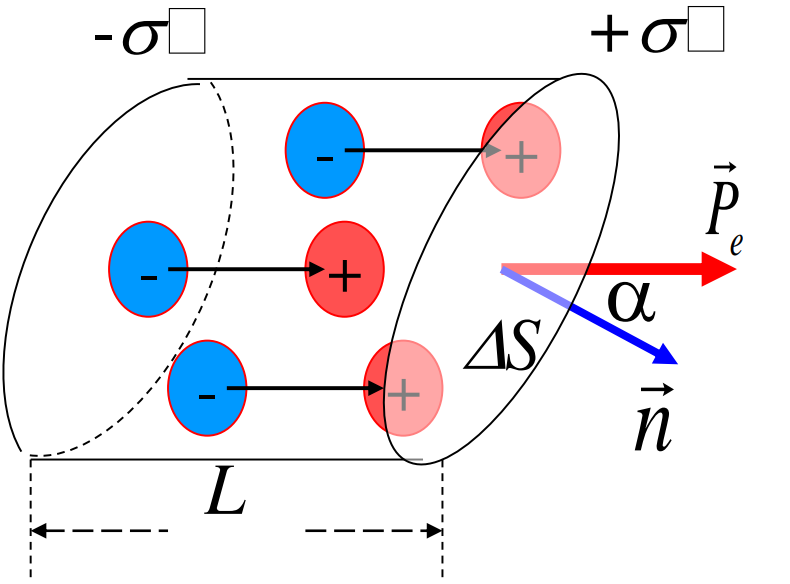
\includegraphics[width=0.5\textwidth]{ch03.png}
\end{figure}

Tách ra khối trụ xiên có

\begin{itemize}
  \item Đường sinh có chiều dài $L$, song song $\vec{E}$
  \item Hai đáy song song có diện tích $\Delta S$
  \item $+\sigma', -\sigma'$ là mật độ điện mặt mỗi đáy
  \item $\vec{n}$ là pháp tuyến của mặt tích điện dương
\end{itemize}

Coi khối trụ xiên như 1 lưỡng cực điện có 2 điện tích $+\sigma' \Delta S$ và $-\sigma' \Delta S$ cách nhau $L$.

\begin{equation*}
  P_e = \left| \vec{P}_e \right| = \frac{\sigma' \Delta S L}{\Delta S L \cos\alpha} = \frac{\sigma'}{\cos\alpha} 
  \Rightarrow \sigma' = P_e\cos\alpha = P_{en}
\end{equation*}

Mật độ điện mặt có giá trị bằng vector phân cực điện môi chiếu lên phương pháp tuyến.

\subsection[Câu 2]{Câu 2: Xác định công thức tính cường độ điện trường tổng hợp trong chất điện môi đồng chất và đẳng hướng. Thế nào là hiệu ứng áp điện thuận và nghịch?}

Tính cường độ điện trường tổng hợp trong điện môi:

\begin{itemize}
  \item Xét điện trường đều $\vec{E}_0$ giữa 2 mp mang điện tích bằng nhau trái dấu
  \item Chất điện môi lấp đầy khoảng giữa
  \item Xảy ra hiện tượng phân cực điện môi, xuất hiện điện tích liên kết $\sigma'$
  \item Điện trường phụ $\vec{E}'$
\end{itemize}

Có $\vec{E} = \vec{E}_0 + \vec{E}' \Rightarrow E = E_0 - E'$

\begin{gather*}
  \begin{cases}
    E' = \frac{\sigma'}{\epsilon_0}\\
    \sigma' = P_{en} = \epsilon_0 \chi_e E
  \end{cases}
  \Rightarrow E' = \chi_e E \\
  E = E_0 - \chi_e E \Rightarrow E = \frac{E_0}{1+\chi_e} = \frac{E_0}{\epsilon}
\end{gather*}

Hiệu ứng áp điện:

\begin{itemize}
  \item Áp điện thuận: Khi nén hoặc kéo giãn một số tinh thể điện môi, xuất hiện điện tích trái dấu
  \item Áp điện nghịch: Khi đặt lên hai mặt của tinh thể một hiệu điện thế thì bị nẽn hoặc giãn
\end{itemize}
\section[Chương 4]{Chương 4: Từ trường}

\subsection[Câu 1]{Câu 1: 
\begin{enumerate}
    \item Thiết lập biểu thức của định luật Ohm dạng vi phân
    \item Trình bày khái niệm nguồn điện và thiết lập biểu thức suất điện động của nguồn điện.
\end{enumerate}
}

\subsubsection{Dạng vi phân của định luật Ôm}

Xét dòng điện trong dây dẫn

\begin{itemize}
  \item Chọn khối trụ nhỏ, dài $dl$, 2 đáy là $dS_n$, vuông góc với $\vec{E}$
  \item Gọi $V$ và $V+dV$ là điện thế ở 2 đáy trụ
\end{itemize}

\begin{gather*}
  dI = \frac{V - (V + dV)}{R} = -\frac{dV}{\rho \frac{dl}{dS_n}} = \frac{E}{\rho} dS_n \\
  \Rightarrow j = \frac{dI}{dS_n} = \frac{E}{\rho} = \sigma E
\end{gather*}

\subsubsection{Nguồn điện}

\begin{itemize}
  \item Xét 2 vật dẫn A mang điện dương, B mang điện âm. Nối AB bằng vật dẫn M
  \item Các hạt dương đi từ $A \to B$, các hạt âm đi từ $B \to A$
  \item Trong vật M xuất hiện dòng điện, đồng thời $V_A$ giảm, $V_B$ tăng. Đến khi $V_A = V_B$ thì dòng dừng
\end{itemize}

Muốn duy trì dòng điện

\begin{itemize}
  \item Đưa các hạt điện dương từ $B \to A$ và $A \to B$. Vì điện trường nên các hạt này không thể tự di chuyển
  \item Phải tác động lực để hạt dương chạy ngược chiều điện trường, hạt âm chạy thuận chiều điện trường
  \item Lực này là lực phi điện tĩnh hay lực lạ
  \item Trường sinh ra lực lạ là trường lạ
  \item Nguồn sinh ra trường lạ là nguồn điện
\end{itemize}

Suất điện động của nguồn điện là đại lượng có giá trị bằng công của lực điện trường để dịch chuyển điện tích $1C$ 1 vòng quanh mạch kín của nguồn đó.

\begin{equation*}
  \zeta = \frac{A}{q}
\end{equation*}

Xét công của lực điện trường tổng hợp $\vec{E} + \vec{E}^*$

\begin{gather*}
  A = \oint q(\vec{E} + \vec{E}^*) d\vec{s} \\
  \zeta = \frac{A}{q} = \oint \vec{E}d\vec{s} + \oint \vec{E}^*d\vec{s} = \oint \vec{E}^*d\vec{s}
\end{gather*}

Suất điện động của nguồn điện có giá trị bằng công của lực lạ để dịch chuyển điện tích $1C$ quanh mạch kín của nguồn đó.

\begin{equation*}
  \zeta = \oint_C \vec{E}^*d\vec{s}
\end{equation*}

\newpage

\subsection[Câu 2]{Câu 2: 
\begin{enumerate}
    \item Phát biểu và viết biểu thức định luật Biot -- Savart -- Laplace, minh họa bằng hình vẽ.
    \item Áp dụng định luật Biot -- Savart -- Laplace tìm cảm ứng từ gây bởi một đoạn dòng điện thẳng tại điểm $M$, cách dòng điện một khoảng $r$; từ đó suy ra biểu thức cho trường hợp dòng điện thẳng dài vô hạn.
\end{enumerate}
}

\subsubsection{Định luật Biot -- Savard -- Laplace}

Vector cảm ứng từ $d\vec{B}$ do một phần tử dòng điện $Id\vec{l}$ gây ra tại điểm $M$ cách một khoảng $\vec{r}$ có

\begin{itemize}
  \item Gốc đặt tại $M$
  \item Phương vuông góc với mặt phẳng chứa $d\vec{l}$ và $\vec{r}$
  \item Chiều sao cho $d\vec{l}, \vec{r}, d\vec{B}$ tạo 1 tam diện thuận (hoặc theo quy tắc vặn nút chai)
  \item Có độ lớn 
  \begin{equation*}
    dB = \frac{\mu_0\mu}{4\pi} \frac{Idl\sin\theta}{r^2}
  \end{equation*}
\end{itemize}

\begin{figure*}[h]
  \centering
  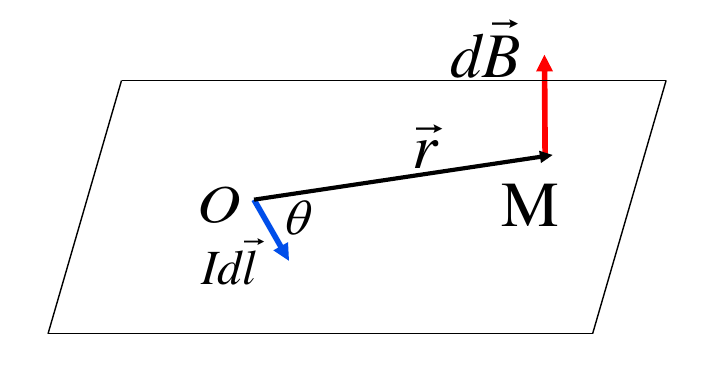
\includegraphics[width=0.4\textwidth]{ch04-1.png}
\end{figure*}

\subsubsection{Áp dụng cảm ứng từ dòng điện thẳng}

\begin{figure}[h]
  \centering
  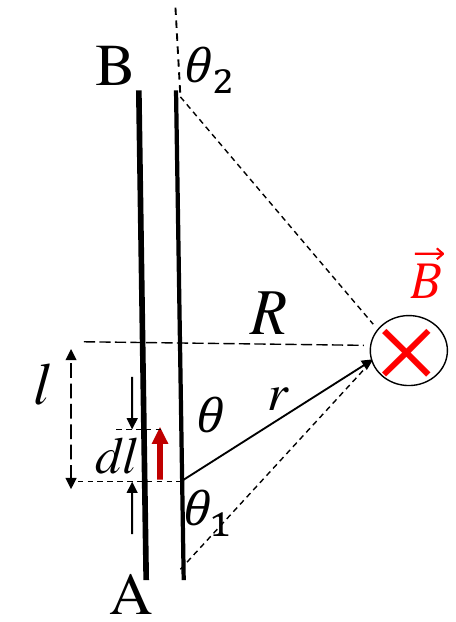
\includegraphics[width=0.4\textwidth]{ch04-2.png}
\end{figure}

\begin{gather*}
  dB = \frac{\mu_0\mu}{4\pi} \frac{Idl\sin\theta}{r^2} \\
  B = \int_{AB} dB = \dots = \frac{\mu_0\mu I}{4\pi R} \left( \cos \theta_1 - \cos \theta_2 \right)
\end{gather*}

Dòng vô tận có 
\begin{equation*}
  B = \frac{\mu_0\mu I}{2\pi R}
\end{equation*}

\subsection[Câu 3]{Câu 3: Xác định vector cảm ứng từ gây bởi dòng điện tròn có cường độ $I$, bán kính $R$, tại điểm $M$ nằm trên trục của dòng điện, cách tâm $O$ của dòng điện một
khoảng $h$. Từ kết quả trên xét hai trường hợp giới hạn:
\begin{itemize}
    \item M trùng với tâm O của dòng điện ($h = 0$)
    \item M ở rất xa dòng điện ($h \gg R$).
\end{itemize}
}

Tính cảm ứng từ gây bởi dòng điện tròn (tự làm):

\begin{equation*}
  \vec{B} = \frac{\mu_0 \mu I \vec{S}}{2\pi (R^2 + h^2)^{\frac{3}{2}}}
\end{equation*}

\begin{itemize}
  \item Ở tâm thì $B = \frac{\mu_0 \mu I}{2R}$
  \item Ở xa thì $B = \frac{\mu_0 \mu IS}{2\pi h^3}$
\end{itemize}

\subsection[Câu 4]{Câu 4: Phát biểu, viết biểu thức và nêu ý nghĩa của định lý Ampe về lưu số của vector cường độ từ trường. Áp dụng định lý Ampe để xác định biểu thức cảm ứng từ trong lòng cuộn dây điện hình xuyến và trong lòng ống dây điện thẳng dài vô hạn mang dòng điện $I$.}

Định lý Ampe về lưu số của vector cường độ từ trường: Lưu số của vector cường độ từ trường dọc theo một đường cong kín bằng tổng đại số cường độ các dòng điện xuyên qua phần diện tích giới hạn bởi đường cong đó.

\begin{equation*}
  \oint_C \vec{H}d\vec{l} = \sum I_i
\end{equation*}

Ý nghĩa: Cho ta biết rằng từ trường là một trường xoáy

\begin{itemize}
  \item Cảm ứng từ trong lòng cuộn dây hình xuyến $n$ vòng, bán kính $R$: $B = \frac{\mu_0 \mu nI}{2\pi R}$
  \item Cảm ứng từ trong lòng cuộn dây dài vô tận: $B = \mu_0\mu n_0I$
\end{itemize}

\subsection[Câu 5]{Câu 5: Trình bày:
\begin{enumerate}
    \item Khái niệm đường sức từ trường
    \item Định nghĩa từ thông qua diện tích $S$
    \item Phát biểu, viết biểu thức và nêu ý nghĩa của định lý O-G đối với từ trường
\end{enumerate}}

\subsubsection{Khái niệm đường sức từ trường}

Đường sức từ trường (hay đường cảm ứng từ) là đường cong trong từ trường mà tiếp tuyến tại mọi điểm trùng với phương của vector cảm ứng từ tại điểm đó, chiều của đường cảm ứng từ là chiều của vector cảm ứng từ

\subsubsection{Định nghĩa từ thông}

Từ thông qua diện tích $dS$ là đại lượng có trị số bằng 

\begin{equation*}
  d\Phi = \vec{B}d\vec{S}
\end{equation*}

Từ thông qua diện tích $dS$ vè trị số là số đường cảm ứng từ qua diện tích ấy.

Tìm từ thông qua diện tích $S$, ta chia thành các diện tích nhỏ $dS$ sao cho $\vec{B}$ trên mỗi diện tích ấy coi như không đổi.

\begin{equation*}
  \Phi = \int_S d\Phi = \int_S \vec{B}d\vec{S}
\end{equation*}

\subsubsection{Định lý O-G trong từ trường}

Từ thông toàn phần gửi qua mặt kín bất kỳ bằng 0

\begin{equation*}
  \oint_S \vec{B}d\vec{S} = 0
\end{equation*}

Ý nghĩa: Từ trường là một trường xoáy. Trong tự nhiên không tồn tại các hạt mang từ tính.

\subsection[Câu 6]{Câu 6: Trình bày tác dụng của từ trường đều lên một mạch điện kín (mạch kín là một khung dây dẫn cứng hình chữ nhật có dòng điện cường độ $I$ chạy qua) trong trường hợp cảm ứng từ hợp với véctơ pháp tuyến mặt phẳng khung một góc $\alpha$.}

\begin{figure}[h]
  \centering
  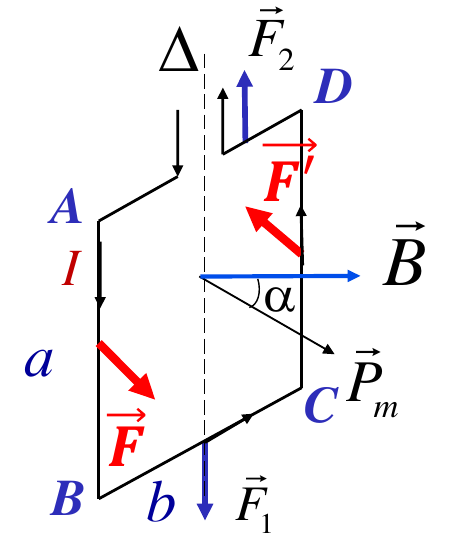
\includegraphics[width=0.4\textwidth]{ch04-3.png}
\end{figure}

Xét khung dây hình chữ nhật có 2 cạnh $a, b$ và dòng $I$

\begin{itemize}
  \item Khung đặt trong từ trường đều $\vec{B}$ có phương vuông góc với $AB, CD$
  \item Khung quay quanh trục $\Delta$
  \item Ban đầu mặt phẳng khung không vuông góc với từ trường
\end{itemize}

Từ lực lên khung có $\sum \vec{F} = \vec{F}_1 + \vec{F}_2 + \vec{F} + \vec{F}'$

\begin{itemize}
  \item $\vec{F}_1 + \vec{F}_2 = \vec{0}$. Phản lực triệt tiêu 
  \item $F = F' = IaB$, tạo thành ngẫu lực khiến khung quay quanh $\Delta$ cho đến khi mặt phẳng khung vuông góc với từ trường
  \item Khung quay theo chiều giảm $\alpha$
\end{itemize}

Khi đó momen ngẫu lực đối với trục $\Delta$ là 

\begin{equation*}
  \mu = Fd = IaB \cdot b\sin\alpha = ISB\sin\alpha = P_m B \sin\alpha
\end{equation*}

Chiều momen ngẫu lực vuông góc với mp chứa $\vec{P}_m$ và $\vec{B}$

\begin{equation*}
  \vec{\mu} = \vec{P}_m \times \vec{B}
\end{equation*}

Năng lượng khung dây trong từ trường:

\begin{equation*}
  W_m(\alpha) = -P_mB\cos\alpha = -\vec{P}_m\vec{B}
\end{equation*}

\subsection[Câu 7]{Câu 7: Trình bày về lực Lorentz tác dụng lên hạt mang điện chuyển động trong từ trường có cảm ứng từ $\vec{B}$. Thành lập phương trình chuyển động của hạt mang điện $q$, khối lượng $m$, chuyển động vận tốc $\vec{v}$ dưới tác dụng của từ trường $\vec{B}$ (góc giữa $\vec{v}$ và $\vec{B}$ là $\alpha$)}

Xét hạt điện $q$ chuyển động với vận tốc $\vec{v}$ trong từ trường $\vec{B}$

\begin{itemize}
  \item Hạt điện chuyển động tương đương phần từ điện tích $Id\vec{l} = q\vec{v}$
  \item Từ lực lên phần tử dòng điện: $d\vec{F} = Id\vec{l} \times \vec{B}$
  \item Lực Lorentz tác dụng lên hạt điện: $\vec{F}_L = q\vec{v} \times \vec{B}$
\end{itemize}

Lực Lorentz: 

\begin{itemize}
  \item Đặt tại hạt điện $q$
  \item Phương vuông góc với phương chuyển động của $q$ và $\vec{B}$
  \item Chiều sao cho $q\vec{v}, \vec{B}, \vec{F}_L$ tạo tam diện thuận
  \item Độ lớn $|F_L| = |q|vB\sin\alpha$
\end{itemize}

Trường hợp chuyển động với góc $\alpha$: Chia $\vec{v}$ thành 2 thành phần $\vec{v}_{//}$ và $\vec{v}_{\perp}$

Khi đó trong mp vuông góc với $\vec{B}$ thì $q$ chuyển động trên đường tròn:

\begin{equation*}
  R = \frac{mv_{\perp}}{|q|B} = \frac{mv\sin\alpha}{|q|B}
\end{equation*}

Quỹ đạo của hạt là hình xoắn ốc với bước

\begin{equation*}
  h = v_{//}T = \frac{2\pi mv\cos\alpha}{|q|B}
\end{equation*}
\section[Chương 5]{Chương 5: Cảm ứng điện từ}

\subsection{Câu 1}

Hiện tượng cảm ứng điện từ là hiện tượng hình thành một suất điện động trên vật dẫn khi vật dẫn được đặt trong một từ trường biến thiên.

Định luật Lenz: Dòng điện cảm ứng sinh ra có chiều sao cho từ trường do nó sinh ra có chiều chống lại nguyên nhân sinh ra nó.

\begin{itemize}
  \item Dịch chuyển 1 vòng dây kim loại trong từ trường để từ thông $\Phi_m$ thay đổi
  \item Trong thời gian $dt$, từ thông biến thiên một lượng $d\Phi_m$
  \item Xuất hiện dòng điện cảm ứng $I_c$
\end{itemize}

Khi đó công của từ lực lên dòng là $dA = I_cd\Phi_m$. Theo định luật Lenz thì công này là công cản (chống lại sự chuyển động). Để dây chuyển động ta cần công $dA'$

\begin{equation*}
  dA' = -dA = -I_cd\Phi_m
\end{equation*}

Công $dA'$ chuyển thành năng lượng của dòng cảm ứng

\begin{equation*}
  E_cI_cdt = -I_cd\Phi_m \Rightarrow E_c = -\frac{d\Phi_m}{dt}
\end{equation*}

Suất điện động cảm ứng bằng về trị số nhưng trái dấu với độ biến thiên của từ thông gửi qua diện tích của mạch.

\subsection{Câu 2}

\subsubsection{Hiện tượng tự cảm}

\begin{itemize}
  \item Ban đầu mạch đóng, điện kế chỉ vị trí $a$
  \item Nếu ngắt mạch thì kim điện kế chạy quá số $0$ rồi mới trở lại
  \item Nếu đóng mạch thì kin điện kế chạy quá $a$ rồi mới trở lại
\end{itemize}

Giải thích:

\begin{itemize}
  \item Khi ngắt mạch, $I$ về 0. Từ thông giảm, trong mạch xuất hiện dòng cảm ứng $I_c$ cùng chiều $I$ để chống lại sự giảm $\Rightarrow$ quá vạch
  \item Khi đóng mạch, $I$ tăng. Từ thông tăng, trong mạch xuất hiện dòng cảm ứng $I_c$ ngược chiều $I$ để chống lại sự tăng $\Rightarrow$ quá vạch
\end{itemize}

Nếu ta thay đổi $I$ trong mạch để từ thông do dòng đó gửi qua diện tích của mạch thay đổi thì trong mạch cũng xuất hiện dòng cảm ứng $I_c$. Vì dòng này do sự cảm ứng dòng trong mạch gây ra nên gọi là hiện tượng tự cảm.

Tính suất điện động tự cảm: Trong mạch đứng yên không đổi hình dạng, suất điện động tự cảm tỉ lệ và trái dấu với độ biến thiên cường độ dòng điện trong mạch.

\begin{equation*}
  E_{tc} = -L\frac{dI}{dt}
\end{equation*}

Xét cuộn dây thẳng dài 

\begin{gather*}
  B = \mu_0\mu \frac{n}{l}I \Rightarrow \Phi = nBS = \mu_0\mu \frac{n^2}{l} IS \\
  \Rightarrow L = \frac{\mu_0\mu n^2 S}{l}
\end{gather*}

\subsubsection{Hiệu ứng bề mặt}

Khi dòng điện cao tần chạy qua 1 dây dẫn thì do hiện tượng tự cảm, dòng điện đó hầu như không chạy trong lòng dây dẫn mà chỉ chạy ở mặt ngoài.

\newpage

\begin{figure*}[h]
  \centering
  \subfloat[\centering]{{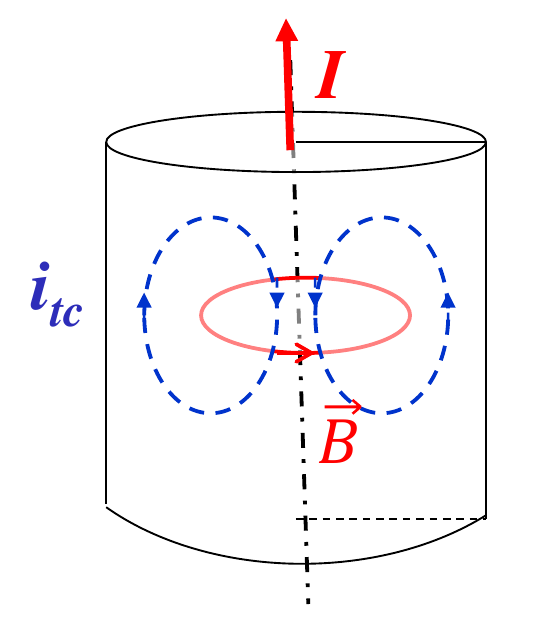
\includegraphics[width=0.3\textwidth]{ch05-1.png}}}
  \qquad
  \subfloat[\centering]{{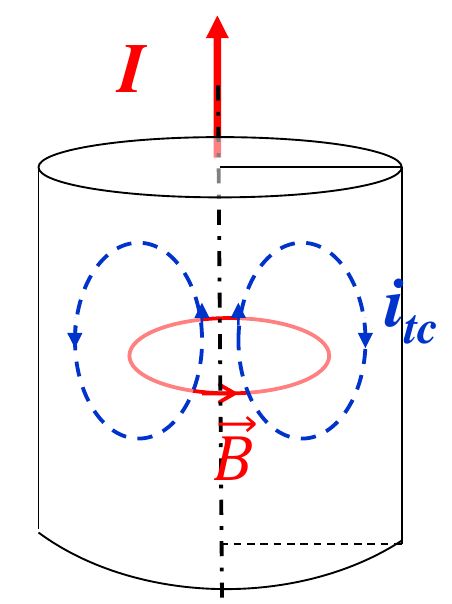
\includegraphics[width=0.3\textwidth]{ch05-2.png}}}
\end{figure*}

Giả sử dòng cao tần đi lên

\begin{itemize}
  \item Dòng $I$ sinh từ trường, biến thiên nên sinh $\vec{B}$ biến thiên
  \item Xét 1 tiết diện $S$ chứa trục đối xứng của dây, $\Phi_m$ qua đó biến thiên, sinh dòng tự cảm khép kín
\end{itemize}

Trong 1/4 chu kì đầu, giả sử dòng đang tăng

\begin{itemize}
  \item $\Phi_m$ qua $S$ tăng, $I_{tc}$ sỉnh $\vec{B}'$ chống lại $\vec{B}$, dòng có chiều như hình (a).
  \item Bên trong thì $I_{tc}$ ngược chiều $I$, dòng giảm
  \item Trên bề mặt $I_{tc}$ cùng chiều $I$, dòng tăng 
\end{itemize}

Trong 1/4 chu kì sau, dòng đang giảm

\begin{itemize}
  \item $\Phi_m$ qua $S$ giảm, $I_{tc}$ sinh $\vec{B}'$ chống lại $\vec{B}$, dòng có chiều như hình (b).
  \item Bên trong thì $I_{tc}$ cùng chiều $I$, dòng mạnh lên
  \item Trên bề mặt $I_{tc}$ ngược chiều $I$, dòng giảm đi
\end{itemize}

Ứng dụng:

\begin{itemize}
  \item Tôi kim loại ở bề mặt
  \item Làm dây dẫn rỗng để tiết kiệm kim loại
\end{itemize}

\subsection{Câu 3}

Áp dụng định lý Ôm trong mạch 

\begin{gather*}
  E + E_{tc} = IR \Rightarrow E = IR + L\frac{dI}{dt} \\
  EIdt = RI^2dt + LIdI
\end{gather*}

Vậy trong quá trình thành lập dòng thì phần năng lượng của nguồn tiềm tàng dưới dạng năng lượng từ trường là

\begin{equation*}
  W_m = \int_{0}^{W_m} dW_m = \int_{0}^{I} LIdI = \frac{1}{2}LI^2
\end{equation*}

Mật độ năng lượng từ trường:

\begin{equation*}
  w_m = \frac{W_m}{V} = \frac{\frac{1}{2}LI^2}{V} = \frac{1}{2} \frac{\mu_0\mu n^2 SI^2}{l^2 S} = \frac{1}{2} \mu_0 \mu \frac{n^2}{l^2} I^2
\end{equation*}

Có $B = \mu_0\mu \frac{n}{l} I$

\begin{equation*}
  w_m = \frac{1}{2} BH
\end{equation*}

Năng lượng từ trường bất kỳ:

\begin{equation*}
  W_m = \int_V w_mdV = \frac{1}{2} \int_V BHdV
\end{equation*}
\section[Chương 6]{Chương 6: Vật liệu từ}

\subsection[Câu 1]{Câu 1: 
\begin{enumerate}
  \item Thế nào là chất nghịch từ, thuận từ, sắt từ?
  \item Trình bày về vecto từ độ $\vec{J}$.
\end{enumerate}
}

\subsubsection{Chất nghịch từ, thuận từ, sắt từ}

Mọi chất đặt trong từ trường đều bị từ hóa. Khi đó chúng trở thành mang từ tính và sinh ra một từ trường phụ $\vec{B}'$. Từ trường tổng hợp $\vec{B}$ trong chất bị từ hóa là 

\begin{equation*}
  \vec{B} = \vec{B}_0 + \vec{B}'
\end{equation*}

\begin{itemize}
  \item Chất nghịch từ: $\vec{B}'$ ngược chiều $\vec{B}_0 \Rightarrow |\vec{B}| < |\vec{B}_0|$ 
  \item Chất thuận từ: $\vec{B}'$ thuận chiều $\vec{B}_0 \Rightarrow |\vec{B}| > |\vec{B}_0|$
  \item Chất sắt từ: $\vec{B}'$ thuận chiều $\vec{B}_0 \Rightarrow |\vec{B}| \gg |\vec{B}_0|$
\end{itemize}

\subsubsection{Từ độ $\vec{J}$}

Vector từ độ là momen từ của một đơn vị thể tích của khối vật liệu từ.

Gọi $\sum \vec{P}_{mi}$ là tổng các momen từ nguyên tử có trong một thể tích $\Delta V$ của vật liệu. Nếu khối vật liệu bị từ hóa đồng đều thì vector từ độ $\vec{J}$ là 

\begin{equation*}
  \vec{J} = \frac{\sum \vec{P}_{mi}}{\Delta V}
\end{equation*}

$J = |\vec{J}|$ là từ độ của vật liệu từ.

Thực nghiệm cho thấy $\vec{J}$ tỉ lệ thuận với từ trường ngoài $\vec{B}_0$.

\begin{equation*}
  \begin{cases}
    \vec{J} = \frac{\chi_m}{\mu_0} \vec{B}_0 \\
    \vec{B}_0 = \mu_0 \vec{H}
  \end{cases}
  \Rightarrow \vec{J} = \chi_m \vec{H}
\end{equation*}

$\chi_m$ là hệ số tỷ lệ phụ thuộc vào bản chất của vật liệu từ và gọi là độ từ hóa của vật liệu từ.

\subsection[Câu 2]{Câu 2: Xây dựng công thức tính cảm ứng từ tổng hợp trong chất thuận từ đồng chất và đẳng hướng.}

\begin{itemize}
  \item Xét khối thuận từ đồng nhất hình trụ dài vô hạn, tiết diện thẳng $S$
  \item Trụ đặt trong từ trường đều $\vec{B}_0$ có phương song song với đường sinh
  \item Giả sử dưới tác dụng của từ trường ngoài, các momen nguyên tử $\vec{P}_m$ nằm dọc theo hướng $\vec{B}_0$
\end{itemize}

Xét các dòng điện nguyên tử trong 1 tiết diện thẳng của trụ:

\begin{itemize}
  \item Bên trong tiết diện thì các dòng điện nguyên tử ngược chiều và triệt tiêu lẫn nhau
  \item Chỉ có các dòng điện nằm dọc trên chu vi của tiết diện là cùng chiều và tạo 1 dòng điện tròn chạy quanh chu vi của tiết diện
\end{itemize}

Vậy nếu xét cả hình trụ thì tất cả các dòng điện nguyên tử trong các tiết diện thẳng sẽ tương đương với 1 dòng điện duy nhất chạy quanh mặt ngoài của trụ như 1 ống dây điện thẳng dài vô hạn.

\begin{itemize}
  \item $n_0$ là số dòng điện tròn trên 1m hình trụ
  \item $i$ là cường độ dòng điện
  \item Cảm ứng phụ sinh ra là $B' = \mu_0 n_0 i$
\end{itemize}

Mặt khác có

\begin{gather*}
  J = \frac{n_0 i S}{S} = n_0 i \\
  \Rightarrow B' = \mu_0 J
\end{gather*}

Vì $\vec{B}'$ thuận chiều $\vec{J} \Rightarrow \vec{B}' = \mu_0 \vec{J}$

Từ trường tổng hợp là 

\begin{equation*}
  \begin{cases}
    \vec{B} = \vec{B}_0 + \mu_0 \vec{J} \\
    \vec{J} = \frac{\chi_m}{\mu_0} \vec{B}_0
  \end{cases}
  \Rightarrow \vec{B} = (1 + \chi_m) \vec{B}_0 = \mu \vec{B}_0 = \mu_0 \mu \vec{H}
\end{equation*}

Lý luận trên cũng đúng với chất nghịch từ.

\begin{itemize}
  \item Thuận từ: $\chi_m > 0 \Rightarrow \mu > 1$
  \item Nghịch từ: $\chi_m < 0 \Rightarrow \mu < 1$
\end{itemize}
\section[Chương 7]{Chương 7: Trường điện từ}

\subsection[Câu 1]{Câu 1: Phát biểu luận điểm 1 của Maxwell. Phân biệt điện trường tĩnh và điện trường xoáy về nguồn gốc phát sinh và tính chất cơ bản. Thiết lập phương trình Maxwell -- Faraday dạng tích phân và vi phân.}

Luận điểm thứ nhất của Maxwell: Bất kỳ từ trường nào biến đổi theo thời gian cũng sinh ra một điện trường xoáy.

Phân biệt điện trường tĩnh và điện trường xoáy:

\begin{table}[H]
\centering
\begin{tabular}{|p{6cm}|p{6cm}|}
\hline
Điện trường tĩnh & Điện trường xoáy \\ \hline\hline
Điện trường tĩnh sinh ra bởi điện tích đứng yên & Điện trường xoáy sinh ra bởi từ trường biến thiên theo thời gian \\ \hline
Là điện trường hở & Là điện trường kín \\ \hline
\end{tabular}
\end{table}

Phương trình Maxwell -- Faraday dạng tích phân:

\begin{equation*}
  \oint_C \vec{E}d\vec{l} = -\frac{d}{dt} \left( \int_C \vec{B}d\vec{S} \right)
\end{equation*}

Lưu số của vector cường độ điện trường dọc theo đường cong kín bất kỳ bằng về trị số nhưng trái dấu với tốc độ biến thiên theo thời gian của từ thông gửi qua diện tích giới hạn bởi đường cong đó.

Phương trình Maxwell -- Faraday dạng vi phân:

\begin{equation*}
  \text{rot}\,\vec{E} = -\frac{\partial\vec{B}}{\partial t}
\end{equation*}

\subsection[Câu 2]{Câu 2: Phát biểu luận điểm 2 của Maxwell. Khái niệm dòng điện dịch. So sánh
dòng điện dịch và dòng điện dẫn. Thiết lập phương trình Maxwell -- Ampere dạng tích phân và vi phân.}

Luận điểm thứ hai của Maxwell: Bất kì một điện trường nào biến đổi theo thời gian cũng sinh ra một từ trường.

Dòng điện dịch là dòng điện tương đương với điện trường biến đổi theo thời gian về phương diện sinh ra từ trường.

Phân biệt dòng điện dẫn và dòng điện dịch:

\begin{table}[H]
\centering
\begin{tabular}{|p{6cm}p{6cm}|}
\hline
\multicolumn{1}{|p{6cm}|}{ Dòng điện dẫn  }& Dòng điện dịch \\ \hline\hline
\multicolumn{1}{|p{6cm}|}{ Là dòng chuyển dời có hướng của các hạt mang điện  }& Là $\vec{E}$ biến thiên theo $t$ \\ \hline
\multicolumn{1}{|p{6cm}|}{ Gây ra tỏa nhiệt theo Joule -- Lenz  }& Không gây ra tỏa nhiệt theo Joule -- Lenz \\ \hline
\multicolumn{2}{|c|}{Đều gây ra từ trường $\vec{B}$} \\ \hline
\end{tabular}
\end{table}

Phương trình Maxwell -- Ampere dạng tích phân:

\begin{equation*}
  \oint_C \vec{H}d\vec{l} = \int_S \left( \vec{J}_{\text{dẫn}} + \frac{\partial \vec{D}}{\partial t} \right) d\vec{S}
\end{equation*}

Lưu số của vector cường độ từ trường dọc theo đường cong kín bất kỳ bằng cường độ dòng điện toàn phần chạy qua diện tích giới hạn bởi đường cong đó.

Phương trình Maxwell -- Ampere dạng vi phân:

\begin{equation*}
  \text{rot}\,\vec{H} = \vec{J}_{\text{dẫn}} + \frac{\partial \vec{D}}{\partial t}
\end{equation*}
\section[Chương 8]{Chương 8: Dao động điện từ}

\subsection[Câu 1]{Câu 1: Thiết lập biểu thức trong dao động điện từ điều hòa.}

Xét mạch $LC$. Trong quá trình dao động năng lượng không đổi: $W_e + W_m = \text{const}$

\begin{align*}
  {}\quad & \frac{1}{2} \frac{q^2}{C} + \frac{1}{2} LI^2 = \text{const} \\
  \Rightarrow\quad & \frac{q}{C} \frac{dq}{dt} + LI \frac{dI}{dt} = 0 \\
  \Rightarrow\quad & \frac{q}{C} + L\frac{dI}{dt} = 0 \\
  \Rightarrow\quad & \frac{d^2I}{dt^2} + \frac{1}{LC} I = 0
\end{align*}

Đặt $\omega_0^2 = \frac{1}{LC}$, ta có $\frac{d^2I}{dt^2} + \omega_0^2 I = 0$

\begin{equation*}
  I = I_0 \cos\left( \omega_0 t + \varphi \right)
\end{equation*}

\subsection[Câu 2]{Câu 2: Thiết lập biểu thức trong dao động điện từ tắt dần.}

Xét mạch $RLC$. Do tỏa nhiệt Joule -- Lenz biên độ giảm dần. 

\begin{itemize}
  \item Trong thời gian $dt$, năng lượng mạch giảm một lượng $-dW$
  \item Nhiệt lượng tỏa ra là $RI^2dt$
\end{itemize}

\begin{align*}
  {}\quad & -dW = RI^2dt \\
  \Rightarrow\quad & -d\left( \frac{1}{2} \frac{q^2}{C} + \frac{1}{2} LI^2 \right) = RI^2dt \\
  \Rightarrow\quad & \frac{q}{C} \frac{dq}{dt} + LI \frac{dI}{dt} = -RI^2 \\
  \Rightarrow\quad & \frac{q}{C} + L\frac{dI}{dt} + RI = 0 \\ 
  \Rightarrow\quad & \frac{1}{C} \frac{dq}{dt} + L\frac{d^2I}{dt^2} + R\frac{dI}{dt} = 0 \\
  \Rightarrow\quad & \frac{d^2I}{dt^2} + \frac{R}{L} \frac{dI}{dt} + \frac{1}{LC} I = 0
\end{align*}

Đặt $\omega_0^2 = \frac{1}{LC}$ và $\beta = \frac{R}{2L}$. Khi đó có $\frac{d^2I}{dt^2} + 2\beta\frac{dI}{dt} + \omega_0^2 I = 0$

\begin{equation*}
  I = I_0 e^{-\beta t} \cos\left( \omega t + \varphi \right)
\end{equation*}

với $\omega = \sqrt{\omega_0^2 - \beta^2}$

\subsection[Câu 3]{Câu 3: Thiết lập biểu thức trong dao động điện từ cưỡng bức.}

Xét thế điện động tuần hoàn gắn với mạch $RLC$

\begin{itemize}
  \item Thế điện động là hàm tuần hoàn theo thời gian: $E = E_0 \sin \Omega t$
  \item Trong thời gian $dt$, nguồn cung cấp năng lượng $EIdt$
  \item Năng lượng này là phần tăng năng lượng điện từ của mạch cùng với nhiệt lượng Joule -- Lenz
\end{itemize}

\begin{align*}
  {}\quad & EIdt = d\left( \frac{1}{2}\frac{q^2}{C} + \frac{1}{2} LI^2 \right) + RI^2dt \\
  \Rightarrow\quad & E_0\sin\Omega t \cdot I = \frac{q}{C} \frac{dq}{dt} + LI\frac{dI}{dt} + RI^2 \\
  \Rightarrow\quad & E_0\sin\Omega t = \frac{q}{C} + L\frac{dI}{dt} + RI \\
  \Rightarrow\quad & \frac{d^2I}{dt^2} + \frac{R}{L} \frac{dI}{dt} + \frac{1}{LC} I = \frac{E_0 \Omega}{L} \cos \Omega t \\
\end{align*}

Đặt $\omega_0^2 = \frac{1}{LC}$ và $\beta = \frac{R}{2L}$. Khi đó $\frac{d^2I}{dt^2} + 2\beta\frac{dI}{dt} + \omega_0^2 I = \frac{E_0 \Omega}{L} \cos \Omega t$

\begin{equation*}
  I = I_0 e^{-\beta t} \cos (\omega t + \varphi) + I_0 \cos \left( \Omega t + \Phi \right)
\end{equation*}

với $I_0 = \frac{E_0}{\sqrt{R^2 + \left( \Omega L + \frac{1}{\Omega C} \right)^2}}$
\section{Ghi chú thêm}

Biểu thức của vector mật độ dòng điện $\vec{j}$:

\begin{equation*}
  \vec{j} = n_0e\vec{v}
\end{equation*}

Điện thế của quả cầu bán kính $R$ tích điện $q$:

\begin{equation*}
  V = \frac{q}{4\pi\epsilon_0\epsilon R}
\end{equation*}

% --- Bibliography ---

% Start a bibliography with one item.
% Citation example: "\cite{williams}".

% \begin{thebibliography}{1}

% \bibitem{williams}
%    Williams, David.
%    \textit{Probability with Martingales}.
%    Cambridge University Press, 1991.
%    Print.

% Uncomment the following lines to include a webpage
% \bibitem{webpage1}
%   LastName, FirstName. ``Webpage Title''.
%   WebsiteName, OrganizationName.
%   Online; accessed Month Date, Year.\\
%   \texttt{www.URLhere.com}

% \end{thebibliography}

% --- Document ends here ---

\end{document}
